\documentclass[12pt, a4paper]{article}
\usepackage[utf8]{inputenc}
\usepackage[T1]{fontenc}
\usepackage{graphicx}
\usepackage{hyperref}
\usepackage{amsmath}
\usepackage{listings}
\usepackage{color}
\usepackage{placeins}
\definecolor{codegreen}{rgb}{0,0.6,0}
\definecolor{codegray}{rgb}{0.5,0.5,0.5}
\definecolor{codepurple}{rgb}{0.58,0,0.82}
\definecolor{backcolour}{rgb}{0.95,0.95,0.92}

\lstdefinestyle{mystyle}{
    backgroundcolor=\color{backcolour},   
    commentstyle=\color{codegreen},
    keywordstyle=\color{magenta},
    numberstyle=\tiny\color{codegray},
    stringstyle=\color{codepurple},
    basicstyle=\footnotesize,
    breakatwhitespace=false,         
    breaklines=true,                 
    captionpos=b,                    
    keepspaces=true,                 
    numbers=left,                    
    numbersep=5pt,                  
    showspaces=false,                
    showstringspaces=false,
    showtabs=false,                  
    tabsize=2
}

\lstset{style=mystyle}

\title{Performance Benchmarking and Transformation Accuracy of Image Transformation on CPU vs. GPU}
\author{Marius Marin}
\date{\today}

\begin{document}

\maketitle

\begin{abstract}
This report details the development and benchmarking of a convolutional neural network model designed to transform CIFAR-10 images into grayscale, resized, and flipped versions. The performance of sequential transformations on a CPU were compared with batch processing on both CPU and GPU. The model's accuracy in replicating ground truth transformations was also evaluated. Insights from Weights \& Biases logs and visual comparisons are included to corroborate my findings.
\end{abstract}

\section{Introduction}
\paragraph{}Efficient image processing is crucial in various applications of computer vision. This study focuses on benchmarking the performance of image transformation tasks on CPU and GPU, as well as the accuracy of these transformations using a custom PyTorch model on the CIFAR-10 dataset.


\section{Model Architecture}
The `TransformationModel` was intentionally designed to be simple, composed of a single convolutional layer that introduces minimal learnable parameters. This design choice was motivated by the nature of the transformation task — which is fundamentally deterministic and does not require a deep or complex model architecture. The convolutional layer acts as a feature enhancer, allowing for a slight adaptation to the input data's peculiarities, which might not be captured by fixed operations alone.

\section{Loss Function}
The Mean Squared Error (MSE) loss function was selected for its propensity to penalize larger errors more severely than smaller ones, which is ideal for a task where precise pixel-wise accuracy is essential. MSE is a natural fit for regression tasks where the goal is to closely approximate a target value — in this case, the pixel values of the transformed images.

\section{Early Stopping}
Early stopping was utilized as a form of regularization to prevent overfitting. By monitoring the validation loss and stopping the training when the loss ceases to decrease, we ensure that the model generalizes well without unnecessarily extending the training process. This approach is particularly beneficial when computational resources are limited or when training larger models.

\section{Benchmarking Methodology}
We benchmarked the model's inference time using different batch sizes on both CPU and GPU (ensuring CUDA synchronization on the GPU). The aim was to determine the batch size at which the model's batch processing outperformed sequential transformations on the CPU. The device's computational capabilities were also taken into account.

\section{Code Snippets}
Below are key snippets from our codebase that illustrate the simplicity and effectiveness of our approach.

\subsection{Model Definition}
\begin{lstlisting}[language=Python, caption=TransformationModel definition]
class TransformationModel(nn.Module):
    def __init__(self):
        super(TransformationModel, self).__init__()
        self.conv = nn.Conv2d(3, 3, kernel_size=3, stride=1, padding=1)

    def forward(self, x):
        x = nnf.relu(self.conv(x))
        x = F.resize(x, size=(28, 28), antialias=True)
        x = F.rgb_to_grayscale(x, num_output_channels=1)
        x = F.hflip(x)
        x = F.vflip(x)
        return x
\end{lstlisting}

\subsection{Early Stopping Mechanism}
\begin{lstlisting}[language=Python, caption=EarlyStopping class]
class EarlyStopping:
    def __init__(self, patience=5, min_delta=0):
        self.patience = patience
        self.min_delta = min_delta
        self.best_loss = None
        self.patience_counter = 0

    def __call__(self, val_loss):
        if self.best_loss is None or val_loss < self.best_loss - self.min_delta:
            self.best_loss = val_loss
            self.patience_counter = 0
        else:
            self.patience_counter += 1
            if self.patience_counter >= self.patience:
                return True
        return False
\end{lstlisting}

\subsection{Loss Function Utilization}
\begin{lstlisting}[language=Python, caption=Training loop snippet showing MSE loss calculation]
for images, ground_truth in train_loader:
    optimizer.zero_grad()
    images = images.to(device)
    ground_truth = ground_truth.to(device)
    outputs = model(images)
    loss = loss_function(outputs, ground_truth)
    loss.backward()
    optimizer.step()
    train_loss += loss.item()
\end{lstlisting}

\subsection{Benchmarking Inference Time}
\begin{lstlisting}[language=Python, caption=Benchmarking inference time with varying batch sizes]
batch_sizes = [10, 50, 100, 200]
for batch_size in batch_sizes:
    sequential_time, model_batch_time = test_inference_time(model, device, batch_size)
    print(f"Sequential transforming time: {sequential_time:.4f} seconds")
    print(f"Model batch processing time: {model_batch_time:.4f} seconds")
\end{lstlisting}

\section{Results}

\begin{figure}[ht]
  \centering
  \begin{minipage}[b]{0.9\textwidth}
    \includegraphics[width=\linewidth]{val_los_asgn7_rn.png}
    \caption{Validation Loss evolution on several runs}
    \label{fig:validation_loss}
  \end{minipage}
\end{figure}


\subsection{Transformation Accuracy}
Consistent across all tests, the model achieved a Mean Squared Error (MSE) of \( 5.9 \times 10^{-5} \), showcasing its high precision in image transformation tasks. Visual inspections of the transformed images corroborated these findings, with the model-generated images displaying a close resemblance to their ground truth counterparts. This visual parity, despite the reduced dimensions and grayscale format, underscores the model's ability to capture and replicate the essential features of the input data.
 

\subsection{Inference Time}
Benchmarking across various environments and batch sizes yielded the following inference times, showcasing the model's enhanced processing speed:

\begin{itemize}
    \item \textbf{PyCharm CPU}:
    \begin{itemize}
        \item Batch size 10: Sequential time - 2.0077s; Model time - 2.0503s.
        \item Batch size 50: Sequential time - 2.1514s; Model time - 1.5603s.
        \item Batch size 100: Sequential time - 1.9046s; Model time - 1.6274s.
        \item Batch size 200: Sequential time - 2.5341s; Model time - 1.6344s.
    \end{itemize}
    
    \item \textbf{Colab CPU}:
    \begin{itemize}
        \item Batch size 10: Sequential time - 2.7822s; Model time - 1.9597s.
        \item Batch size 50: Sequential time - 3.2753s; Model time - 1.5744s.
        \item Batch size 100: Sequential time - 2.4885s; Model time - 1.5125s.
        \item Batch size 200: Sequential time - 3.4444s; Model time - 1.5173s.
    \end{itemize}
    
    \item \textbf{Colab T4 GPU}:
    \begin{itemize}
        \item Batch size 10: Sequential time - 3.1330s; Model time - 2.3993s.
        \item Batch size 50: Sequential time - 3.0265s; Model time - 1.6880s.
        \item Batch size 100: Sequential time - 3.5728s; Model time - 2.4954s.
        \item Batch size 200: Sequential time - 2.9728s; Model time - 1.6241s.
    \end{itemize}
\end{itemize}

These results showcase the advantages of batch processing using GPU acceleration, confirming that even with a straightforward convolutional neural network, it is possible to achieve both high accuracy and efficiency in image transformation tasks.

\section{Image Comparisons}
A selection of image comparisons is provided, which includes the model's output and the ground truth transformations.

Below are pairs of images showcasing the transformation accuracy of the model. On the left is the image processed by the model, and on the right is the corresponding ground truth image.

% 1
\begin{figure}[ht]
  \centering
  \begin{minipage}[b]{0.3\textwidth}
    
\includegraphics[width=\linewidth]{original_image_2316.png}
    \caption{Original}
    \label{fig:original_1}
  \end{minipage}
  \hfill
  \begin{minipage}[b]{0.3\textwidth}
    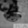
\includegraphics[width=\linewidth]{processed_image_2316.png}
    \caption{Processed by model}
    \label{fig:processed_1}
  \end{minipage}
  \hfill
  \begin{minipage}[b]{0.3\textwidth}
    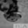
\includegraphics[width=\linewidth]{ground_truth_image_2316.png}
    \caption{Ground truth}
    \label{fig:ground_truth_1}
  \end{minipage}
\end{figure}

% 2
\begin{figure}[ht]
  \centering
  \begin{minipage}[b]{0.3\textwidth}
    
\includegraphics[width=\linewidth]{original_image_2951.png}
    \caption{Original}
    \label{fig:original_2}
  \end{minipage}
  \hfill
  \begin{minipage}[b]{0.3\textwidth}
    
\includegraphics[width=\linewidth]{processed_image_2951.png}
    \caption{Processed by model}
    \label{fig:processed_2}
  \end{minipage}
  \hfill
  \begin{minipage}[b]{0.3\textwidth}
    
\includegraphics[width=\linewidth]{ground_truth_image_2951.png}
    \caption{Ground truth}
    \label{fig:ground_truth_2}
  \end{minipage}
\end{figure}

% 3
\begin{figure}[ht]
  \centering
  \begin{minipage}[b]{0.3\textwidth}
    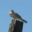
\includegraphics[width=\linewidth]{original_image_3652.png}
    \caption{Original}
    \label{fig:original_3}
  \end{minipage}
  \hfill
  \begin{minipage}[b]{0.3\textwidth}
    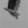
\includegraphics[width=\linewidth]{processed_image_3652.png}
    \caption{Processed by model}
    \label{fig:processed_3}
  \end{minipage}
  \hfill
  \begin{minipage}[b]{0.3\textwidth}
    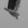
\includegraphics[width=\linewidth]{ground_truth_image_3652.png}
    \caption{Ground truth}
    \label{fig:ground_truth_3}
  \end{minipage}
\end{figure}

% 4
\begin{figure}[ht]
  \centering
  \begin{minipage}[b]{0.3\textwidth}
    
\includegraphics[width=\linewidth]{original_image_4032.png}
    \caption{Original}
    \label{fig:original_4}
  \end{minipage}
  \hfill
  \begin{minipage}[b]{0.3\textwidth}
    
\includegraphics[width=\linewidth]{processed_image_4032.png}
    \caption{Processed by model}
    \label{fig:processed_4}
  \end{minipage}
  \hfill
  \begin{minipage}[b]{0.3\textwidth}
    
\includegraphics[width=\linewidth]{ground_truth_image_4032.png}
    \caption{Ground truth}
    \label{fig:ground_truth_4}
  \end{minipage}
\end{figure}

% 5
\begin{figure}[ht]
  \centering
  \begin{minipage}[b]{0.3\textwidth}
    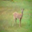
\includegraphics[width=\linewidth]{original_image_4683.png}
    \caption{Original}
    \label{fig:original_5}
  \end{minipage}
  \hfill
  \begin{minipage}[b]{0.3\textwidth}
    
\includegraphics[width=\linewidth]{processed_image_4683.png}
    \caption{Processed by model}
    \label{fig:processed_5}
  \end{minipage}
  \hfill
  \begin{minipage}[b]{0.3\textwidth}
    
\includegraphics[width=\linewidth]{ground_truth_image_4683.png}
    \caption{Ground truth}
    \label{fig:ground_truth_5}
  \end{minipage}
\end{figure}

% 6
\begin{figure}[ht]
  \centering
  \begin{minipage}[b]{0.3\textwidth}
    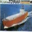
\includegraphics[width=\linewidth]{original_image_6379.png}
    \caption{Original}
    \label{fig:original_6}
  \end{minipage}
  \hfill
  \begin{minipage}[b]{0.3\textwidth}
    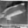
\includegraphics[width=\linewidth]{processed_image_6379.png}
    \caption{Processed by model}
    \label{fig:processed_6}
  \end{minipage}
  \hfill
  \begin{minipage}[b]{0.3\textwidth}
    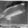
\includegraphics[width=\linewidth]{ground_truth_image_6379.png}
    \caption{Ground truth}
    \label{fig:ground_truth_6}
  \end{minipage}
\end{figure}

% 7
\begin{figure}[ht]
  \centering
  \begin{minipage}[b]{0.3\textwidth}
    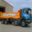
\includegraphics[width=\linewidth]{original_image_6891.png}
    \caption{Original}
    \label{fig:original_7}
  \end{minipage}
  \hfill
  \begin{minipage}[b]{0.3\textwidth}
    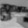
\includegraphics[width=\linewidth]{processed_image_6891.png}
    \caption{Processed by model}
    \label{fig:processed_7}
  \end{minipage}
  \hfill
  \begin{minipage}[b]{0.3\textwidth}
    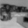
\includegraphics[width=\linewidth]{ground_truth_image_6891.png}
    \caption{Ground truth}
    \label{fig:ground_truth_7}
  \end{minipage}
\end{figure}

% 8
\begin{figure}[ht]
  \centering
  \begin{minipage}[b]{0.3\textwidth}
    
\includegraphics[width=\linewidth]{original_image_8717.png}
    \caption{Original}
    \label{fig:original_8}
  \end{minipage}
  \hfill
  \begin{minipage}[b]{0.3\textwidth}
    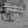
\includegraphics[width=\linewidth]{processed_image_8717.png}
    \caption{Processed by model}
    \label{fig:processed_8}
  \end{minipage}
  \hfill
  \begin{minipage}[b]{0.3\textwidth}
    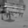
\includegraphics[width=\linewidth]{ground_truth_image_8717.png}
    \caption{Ground truth}
    \label{fig:ground_truth_8}
  \end{minipage}
\end{figure}

% 9
\begin{figure}[ht]
  \centering
  \begin{minipage}[b]{0.3\textwidth}
    
\includegraphics[width=\linewidth]{original_image_9110.png}
    \caption{Original}
    \label{fig:original_9}
  \end{minipage}
  \hfill
  \begin{minipage}[b]{0.3\textwidth}
    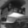
\includegraphics[width=\linewidth]{processed_image_9110.png}
    \caption{Processed by model}
    \label{fig:processed_9}
  \end{minipage}
  \hfill
  \begin{minipage}[b]{0.3\textwidth}
    
\includegraphics[width=\linewidth]{ground_truth_image_9110.png}
    \caption{Ground truth}
    \label{fig:ground_truth_9}
  \end{minipage}
\end{figure}

% 10
\begin{figure}[ht]
  \centering
  \begin{minipage}[b]{0.3\textwidth}
    
\includegraphics[width=\linewidth]{original_image_9374.png}
    \caption{Original}
    \label{fig:original_10}
  \end{minipage}
  \hfill
  \begin{minipage}[b]{0.3\textwidth}
    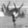
\includegraphics[width=\linewidth]{processed_image_9374.png}
    \caption{Processed by model}
    \label{fig:processed_10}
  \end{minipage}
  \hfill
  \begin{minipage}[b]{0.3\textwidth}
    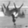
\includegraphics[width=\linewidth]{ground_truth_image_9374.png}
    \caption{Ground truth}
    \label{fig:ground_truth_10}
  \end{minipage}
\end{figure}

\FloatBarrier %
\section{Conclusion}
Batch processing, especially on GPUs, can greatly enhance the efficiency of image transformation tasks. The developed model serves as a testament to the potential of simple architectures in achieving high accuracy in such tasks.


\end{document}
